\chapter{Študije primerov}

\section{Primer za učenje jezikov}

\subsection{Opis problema}

Prvi primer je preprosta grafična aplikacija, ki uporabnikom olajša učenje tujih jezikov. Deluje na preprostem principu pomnjenja besed. Igralcu se na zaslonu pokaže beseda v domačem jeziku in tri besede v jeziku, ki se ga uporabnik skuša naučiti. Dve besedi od treh tujih sta naključno izbrani, tretja pa je pravilni odgovor.

V primeru pravilnega odgovora se uporabniku pokaže naslednja beseda in trije novi odgovori. Tako uporabnik nadaljuje z učenjem. Če uporabnik izbere napačni odgovor, se na zaslonu pojavi pravilni prevod besede, tako da se ima uporabnik možnost naučiti besedo. Ko si uporabnik ogleda pravilni odgovor se igra ponastavi ter začne od začetka.

Na sliki \ref{german} je glavni zaslon aplikacije s tremi možnimi odgovori.

\begin{figure}
\begin{center}
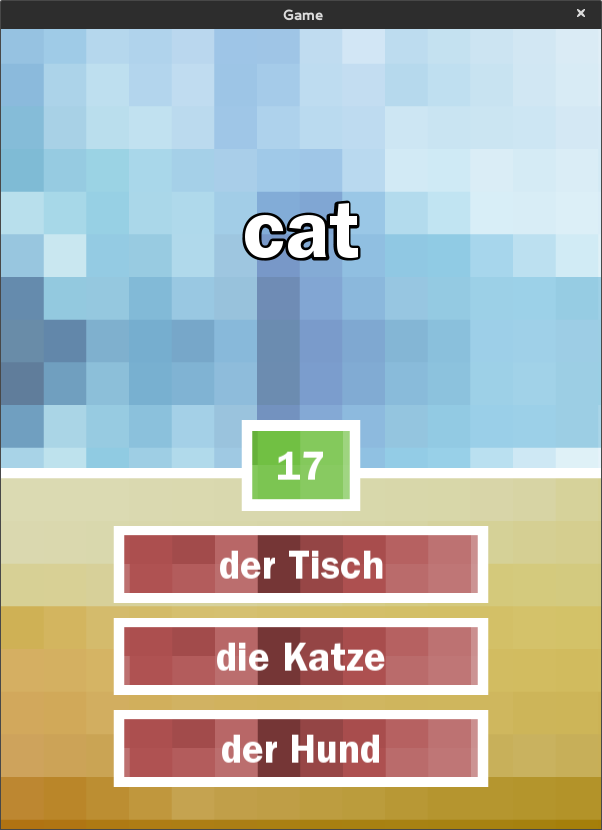
\includegraphics[width=5.5cm]{pic/defg-german.png}
\end{center}
\caption{Primer delovanja Nemške verzije na mobilni napravi}
\label{german}
\end{figure} 

Ena izmed glavnih zahtev igre je izpis različnih pisav in posebnih znakov. Poleg prikazane verzije nemščina-angleščina, je bila aplikacija razvita tudi z idejo učenja jezikov, ki ne uporabljajo latinice. Slika \ref{korean} prikazuje primer učenja Korejščine. Aplikacije mora biti sposobna izrisovati velik nabor različnih abeced.

\begin{figure}
\begin{center}
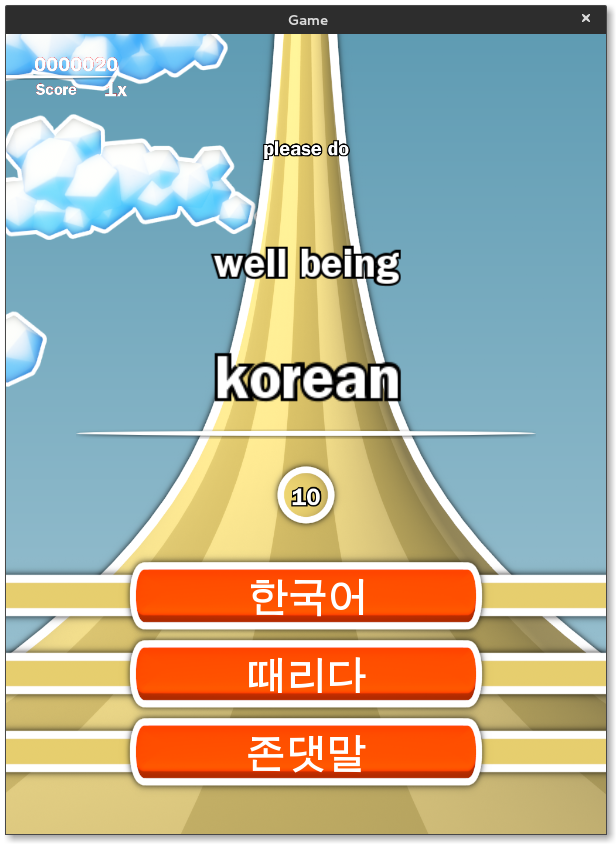
\includegraphics[width=5.5cm]{pic/defg-korean.png}
\end{center}
\caption{Primer delovanja Korejske verzije na namiznem računalniku}
\label{korean}
\end{figure} 

Aplikacija je bila zamišljena kot mobilna aplikacijam za platformi iOS in Android, vendar je zelo uporabno imeti možnost razvoja in izvajanja na namiznem računalniku. Zato smo se odločili za metodo PlayN.

\subsection{Uporabljena metoda}

Izmed vseh obravnavanih metod se nam je zdela najbolj primerna metoda PlayN. Razlogi za izbiro metode so naslednji:

\begin{itemize}
\item PlayN je odprto koden projekt. V primeru težav lahko pogledamo v izvorno kodo projekta in po potrebi težave odpravimo sami.
\item Licenca, ki jo PlayN uporablja, ni omejujoča in v primerjavi z nekaterimi plačljivimi metodami, ne zahteva nobenega plačila pred uporabo. To velja tudi, če bi aplikacijo uporabili za komercialne namene.
\item PlayN je še vedno v aktivnem razvoju, razvijalci pa so odzivni na listi za elektronsko pošto.
\item Orodje PlayN omogoča preprosto podporo dodajanju lastnih pisav, kar je ključnega pomena za podporo jezikom, kot je Korejščina.
\item Število platform, ki jih PlayN podpira, zadošča potrebam aplikacije.
\item PlayN omogoča uporabo vročega izmenjevanja kode, kar zelo pohitri razvoj aplikacije.
\item Poleg samega ogrodja PlayN je na voljo tudi precej vtičnikov, ki so jih napravili uporabniki. Tak primer je vtičnik Tripleplay, ki je v aplikaciji uporabljen za prikaz menijev.
\item Dokumentacija je dobro napisana in razumljiva.
\end{itemize}

Izbira je potekala med PlayN in podobno knjižnico LibGDX. Na koncu smo se odločili za PlayN zaradi lažje uporabe lastnih pisav v aplikaciji. O uporabi plačljivih rešitev nismo razmišljali.

\subsection{Opis metode}

Projekt z uporabo pogona PlayN sestavlja več imenikov. Glavni imenik se imenuje $core$ in vsebuje logiko celotne aplikacije. Izvorna koda, ki se nahaja v tem imeniku, definira kaj se bo na zaslonu prikazalo ter kako se aplikacija odziva na vnose uporabnikov. 

Imenik $assets$ služi kot imenik vseh sredstev, ki jih aplikacija potrebuje za delovanje. V imeniku se nahaja vsa grafika, ki je v uporabi v igri, in vse zvočne datoteke.

Ostali imeniki so namenjeni posameznim platformam. Imenik $java$ vsebuje preprost program, ki odpre okno in nastavi grafično okolje. Ko je okno pripravljeno pokliče glavno metodo imenika $core$ in aplikacija se začne izvajati. Slično delujeta tudi imenika $android$ in $ios$, vsak za svojo platformo. Oba definirata vse potrebno za zagon na sistemih Android in iOS in nato pokličeta metodo iz imenika $core$.

\subsection{Prednosti izbora metode}

Izbrana metoda nam je pomagala izpolniti vse zastavljene cilje. Brez truda smo aplikacijo razvijali na miznem računalniku in po potrebi preizkusili delovanje na Android napravi. Vmesnik API je razumljiv in krivulja učenja ni bila strma. 

\subsection{Slabosti izbora metode}

Težave smo imeli pri testiranju verzije za iOS naprave. Kljub izčrpni dokumentaciji smo naleteli na probleme s konflikti med pritiklinami ogrodja PlayN. Z nekaj raziskovanja nam je vse probleme uspelo odpraviti. 

Nekaj težav je povzročil tudi prehod na novo verzijo iz 1.6 na 1.7, ki se je zgodil med razvojem aplikacije. Nova verzija je malce spremenila način dela s sredstvi in potrebnih je bilo nekaj ročnih popravkov, da sta Android in iOS verziji ponovno delovali.

\section{Primer štiri v vrsto}

Testna aplikacija je preprosta igra štiri v vrsto postavljena v treh dimenzijah. Ideja aplikacije je skozi preprosto igro izboljšati uporabnikovo orientacijo v 3D prostoru. Za razliko od standardne igre štiri v vrsto, kjer so zmagovalne kombinacije omejene v vodoravni, navpični in horizontalni smeri, imamo v 3D verziji veliko več možnosti. Poleg osnovnih smeri lahko zmagovalno kombinacijo zgradimo tudi v globino, kar odpre obilico novih kombinacij.

\subsection{Uporabljena metoda}

Za razvoj smo se odločili za orodje Unity. Unity za razliko od ostalih metod, ki smo  jih ogledali, Unity vključuje svoje integrirano razvojno okolje, ki ga prikazuje slika \ref{mineditor}. Urejevalnik nam omogoča grajenje objektov, postavitev kamere in določitev luči. Za postavitev objektov v 3D prostor se uporablja okno z ortografsko ali perspektivno projekcijo ter različnimi možnimi pogledi. Slika \ref{minplay} prikazuje delovanje aplikacije na mobilni platformi Nexus 7.

\begin{figure}
\begin{center}
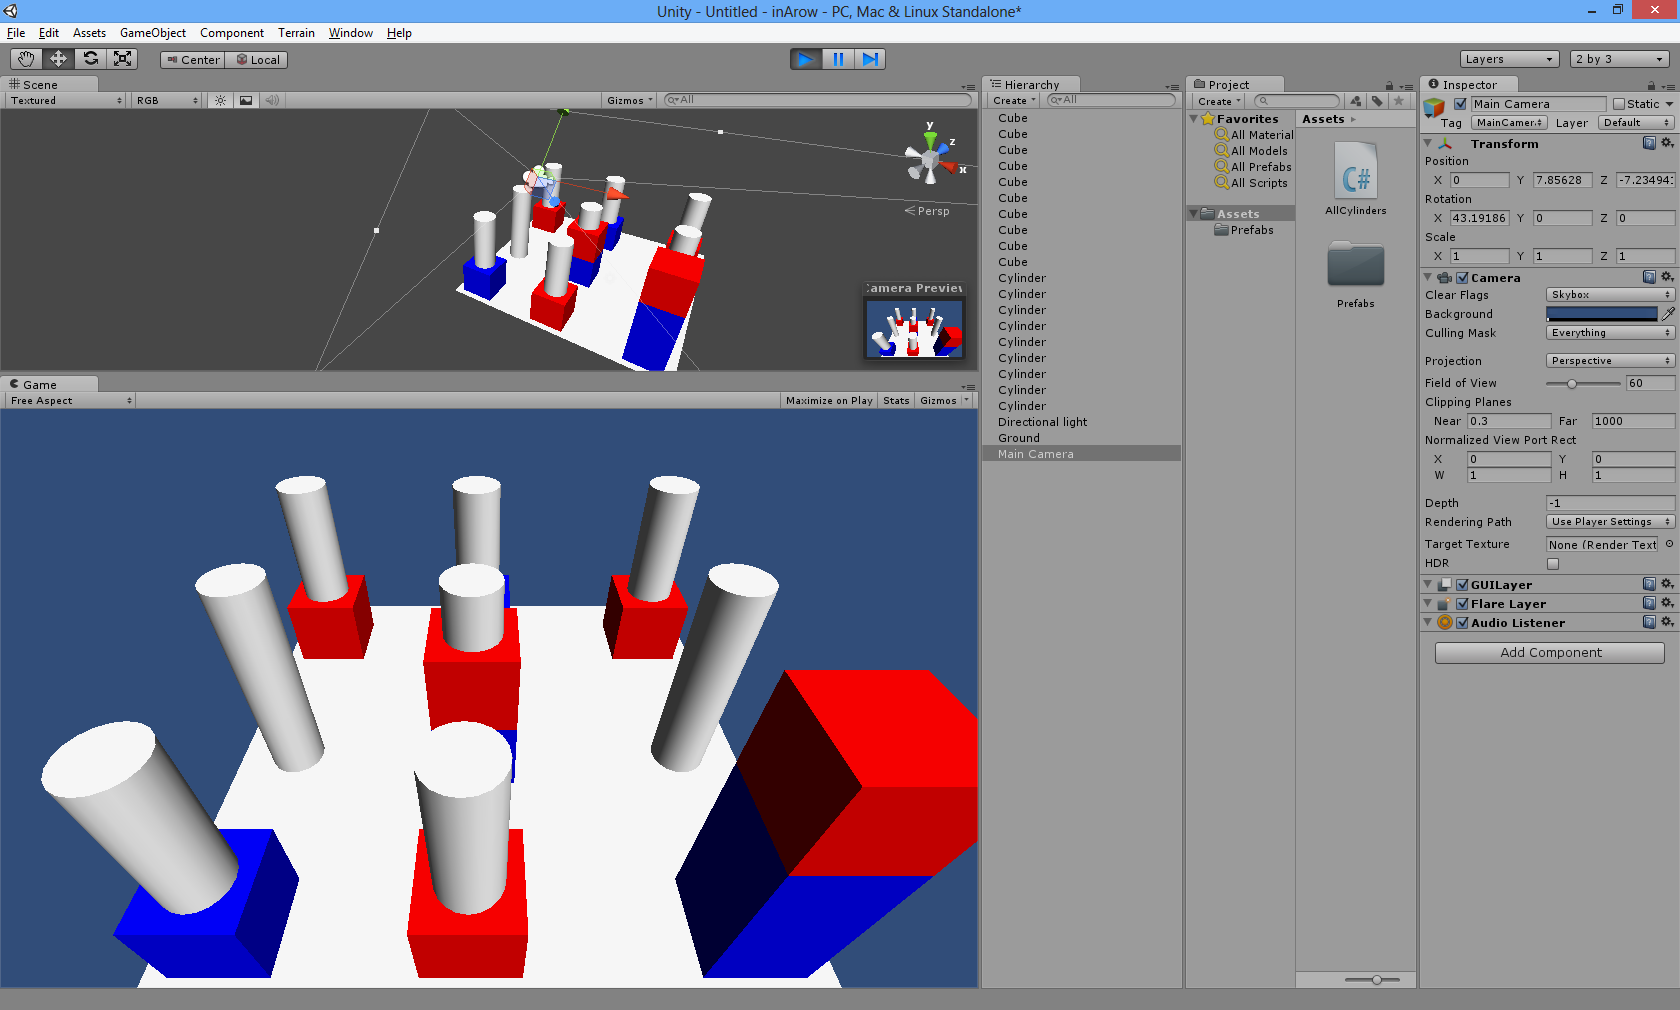
\includegraphics[width=12cm]{pic/min-editor.png}
\end{center}
\caption{Razvoj grafično intenzivne aplikacije v okolju Unity.}
\label{mineditor}
\end{figure} 

\begin{figure}
\begin{center}
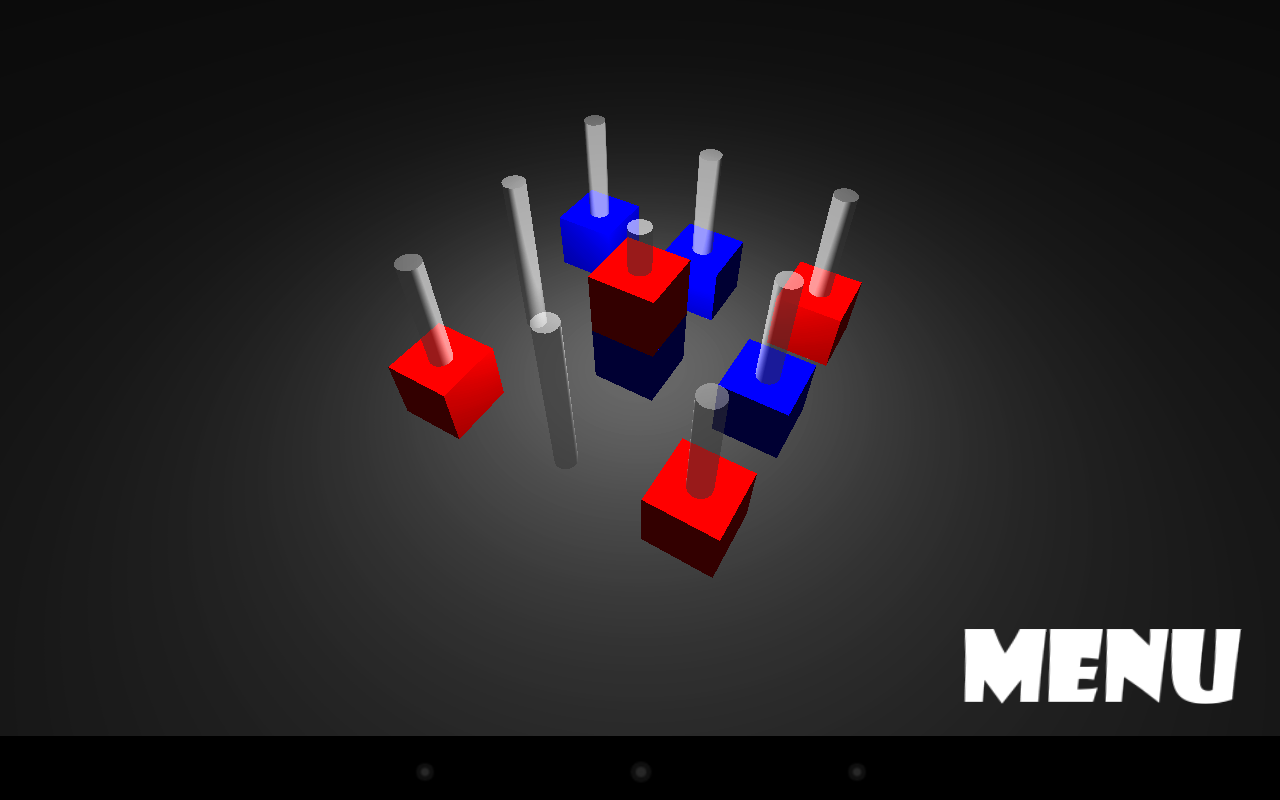
\includegraphics[width=10cm]{pic/min-play.png}
\end{center}
\caption{Končana Unity aplikacija izvožena na mobilno platformo.}
\label{minplay}
\end{figure} 

S pomočjo uporabniškega vmesnika določimo pozicije objektov, materiale in druge lastnosti. Za logiko, obnašanje in odziv na uporabniški vhod pa vsakemu objektu lahko dodelimo tudi skriptno datoteko. V tej skriptni datoteki v enem od podprtih programskih jezikih (C\#, JavaScript, Boo) določimo kako se bo objekt odzival na uporabniški vhod in določimo kako se bo obnašal v času, ko je viden na zaslonu.

Aplikacija je zasnovana preprosto. Ko se igra zažene se ustvarijo prazni valji, na katere se nastavi dogodek $addBlock$, ki se sproži ob dotiku na valj. Unity okolje avtomatično prevede koordinate zaslona v koordinate prostora in pravilno preveli, katerega stolpa smo se dotaknili. Prav tako orodje Unity abstrahira način dotika, le ta je lahko klik z miško ali pa dotik na dotik občutljivem zaslonu.

Dogodek $addBlock$ na izbrani valj položi novo barvasto kocko - rdečo ali modro, odvisno kateri igralec je na voljo. Nova kocka se tudi doda na seznam, ki interno predstavlja stanje igralne plošče. Algoritem nato preveri novo stanje seznama, če se je z novo potezo pojavila zmagovalna kombinacija.

Če se je igra končala, se pojavi besedilo, ki sporoči zmagovalca in ponudi ponovno igranje. V bolj pogostem primeru, ko poteza ne zaključi igre, se samo zamenja aktivni igralec in igra se nadaljuje. 

\subsection{Prednosti metode}

Unity urejevalnik nam je omočil zelo hiter razvoj aplikacije, saj je bilo ustvarjanje osnovnih oblik in postavitev le teh v prostor, zelo preprosto. Pisanje skriptnih datotek za obnašanje in logiko aplikacije tudi ni bilo težavno.

\subsection{Slabosti metode}

Problem uporabe orodja Unity je učna krivulja. Za razliko od večine ostalih metod, se moramo poleg vmesnika API naučiti tudi dela s priloženim urejevalnikom. Sicer je urejevalnik preprost za uporabo, vendar učenje vseh potrebnih operacij vzame precej časa.

Druga slabost metode je v zaprtost sistema. Če tekom razvoja aplikacije naletimo na omejitev orodja nimamo dostopa do izvorne kode, kjer bi to omejitev lahko odpravili. Orodje je sicer na voljo brezplačno, vendar moramo za uporabo naprednih funkcij plačati za licenco. Aplikacije razvite z brezplačno verzijo programa imajo na vseh platformah pred zagonom zaslon z napisom Unity. 

\section{Primer MIN (WebGL)}

Primer MIN je preprosta igra z ortografsko projekcijo. Cilj igre je odstraniti rdeče kocke s sivo kocko, ki jo premika igralec. Premikanje sive kocke levo, desno, navzgor in navzdol je možno samo v naprej določenih perspektivah. V ptičji perspektivi, kjer vidimo pozicije vseh rdečih kock, premikanje sploh ni možno. V drugi perspektivi se lahko premikamo samo levo in desno, zaradi ortografske projekcije pa ne ločimo katere kocke so višje ali nižje nad nami. V tretji perspektivi pa se lahko premikamo navzgor in navzdol, ne vidimo pa več katere kocke so levo in katere desno od nas. Če se med spreminjanjem perspektive siva kocka dotakne črne črte, se igrana stopnja ponastavi. Slika \ref{minff} prikazuje delovanje končane aplikacije v mobilnem brskalniku.

\begin{figure}
\begin{center}
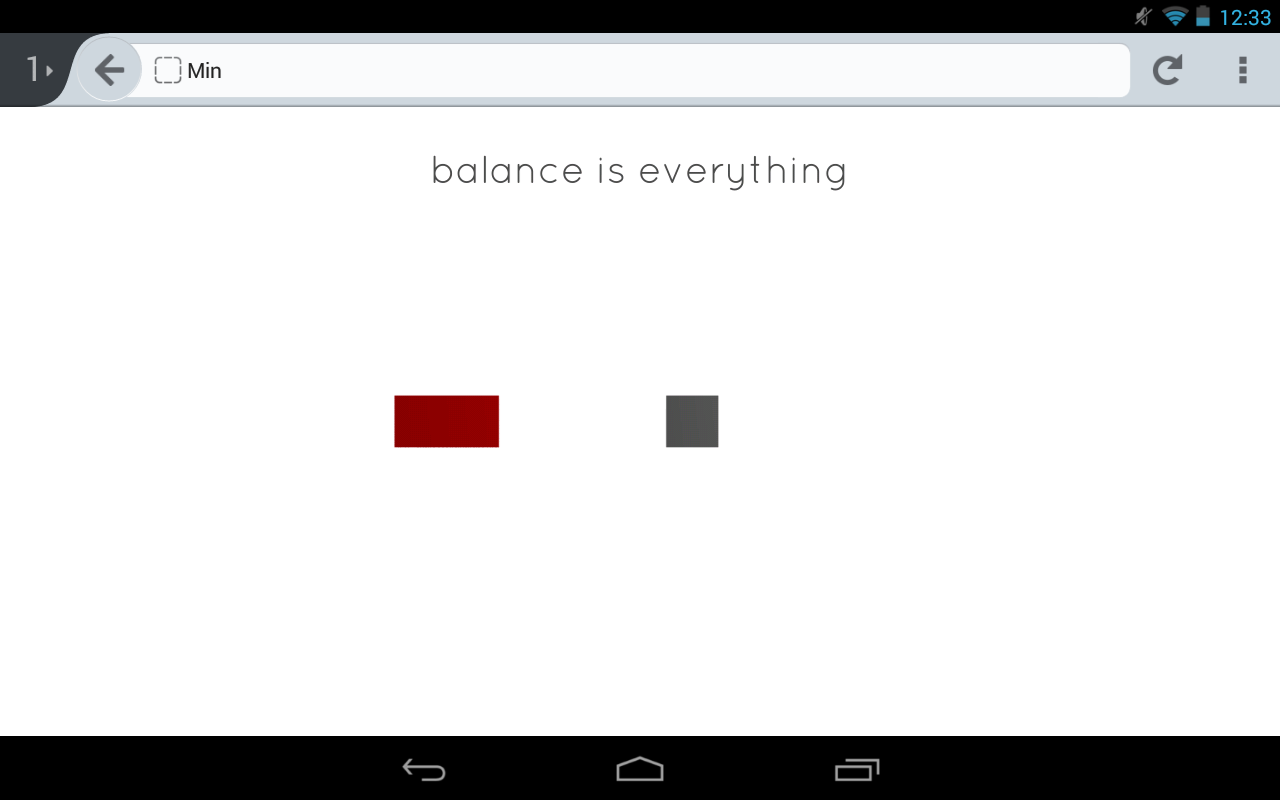
\includegraphics[width=12cm]{pic/min-ff.png}
\end{center}
\caption{Delovanje igre v mobilnem brskalniku Firefox.}
\label{minff}
\end{figure}

\subsection{Uporabljena metoda}

Aplikacije smo se razvili kot spletno aplikacijo, ki uporablja tehnologijo WebGL. WebGL omogoča strojno pospeševanje, kar pomaga pri animaciji za preklop med perspektivami. Ta uporabniku daje občutek 3D prostora. Razen te animacije, bi lahko vse ostale dele aplikacije brez problema realizirali z uporabo 2D platna.

Za lažje delo z WebGLom smo uporabili knjižnico THREE.js, ki poenostavi delo s 3D objekti. Uporabili smo tudi knjižnico hammer.js, ki nam pomaga zaznavati geste na dotik občutljivem zaslonu.


\subsection{THREE.js}

THREE.js je knjižnica za delo z WebGLom. Ponudi nam pester nabor uporabnih metod, ki močno poenostavijo izrisovanje modelov, določanje materialov, postavitev kamere in raznoraznih luči v sceno. Knjižnica pripravi tudi potrebne senčilnike tako da uporabniku ni potrebno pisati GLSL izvorne kode, vse potrebno lahko opravi z Javascriptom. Pisanje lastnih GLSL programov je vseeno možno.

\subsection{hammer.js}

Hammer.js je Javascript knjižnica za zaznavanje gest. Okoli standardnih dogodkov, ki se v brskalnikih sprožijo na dotik zgradi lastne funkcije, ki posamezne dogodke znajo združiti v geste. Tako uporabniku ni potrebno pisati izvorne kode, ki iz posameznik dogodkov na primer zazna gesto za poteg v desno.

Knjižnica omogoča naročanje na dogodke tipa poteg desno. Primer izvorne kode, ki se naroči na ta dogodek vidimo v Primeru \ref{swipeleft}.

Hammer(element).on(\"swipeleft", function(event){ ... }); 

Na podoben način se lahko naročimo tudi na druge vrste dogodkov, med katere spadajo potegi v vse možne smeri, daljši pritisk, kratek pritisk, uščipni za povečavo in tako naprej.

Knjižnica omogoča tudi nastavitve posameznih gest, kot so dolžina pritiska potrebna za dogodek daljši pritisk, ...

\subsection{Prednosti izbora metode}

Izbrana metoda nam je omogočila hiter razvoj aplikacije. Aplikacijo smo razvijali na namiznem računalniku, kjer moderni brskalniki (Chrome, Firefox) podpirajo celo simuliranje dogodkov, ki se sprožajo na zaslonih občutljivih na dotik. Potrebe po testiranju na mobilni napravi je bilo zelo malo. V tem primeru smo delovanje na tabličnem računalniku Nexus 7 preizkusili šele, ko je bila celotna aplikacija končana, s kodo, ki zaznava dotik dogodke.

\subsection{Slabosti izbora metode}

Glavna slabost metode je slaba podpora na mobilnih brskalnikih. Mobilni brskalnik Firefox je sicer prikazal našo aplikacijo pravilno, vendar smo morali za delovanje v brskalniku Chrome omogočiti posebno nastavitev. Slika \ref{minchromeflag} prikazuje zaslon, kjer se nastavi zastavica za omogočanje WebGLa. Po vključimo zastavico aplikacija deluje pravilno, kot kaže tudi \ref{minchrome}. Dokler podjetje Google privzeto ne omogoči te zastavice, WebGL aplikacije ne bodo primerne za navadne uporabnike. 

\begin{figure}
\begin{center}
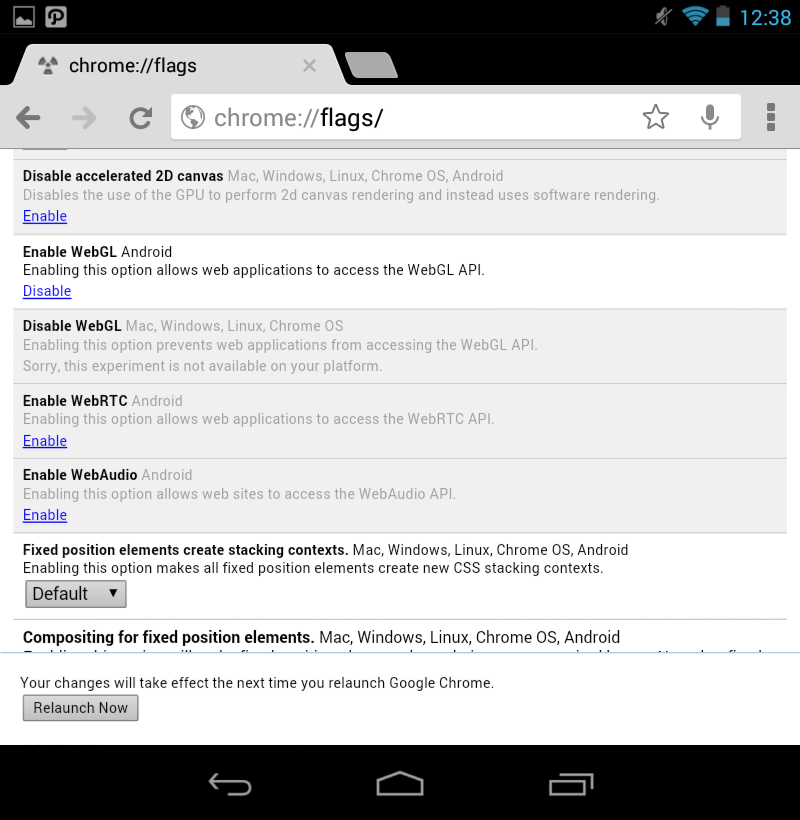
\includegraphics[width=10cm]{pic/min-chrome-flag.png}
\end{center}
\caption{Za delovanje v brskalniku Chrome na Androidu je potrebno nastaviti posebno zastavico.}
\label{minchromeflag}
\end{figure} 

\begin{figure}
\begin{center}
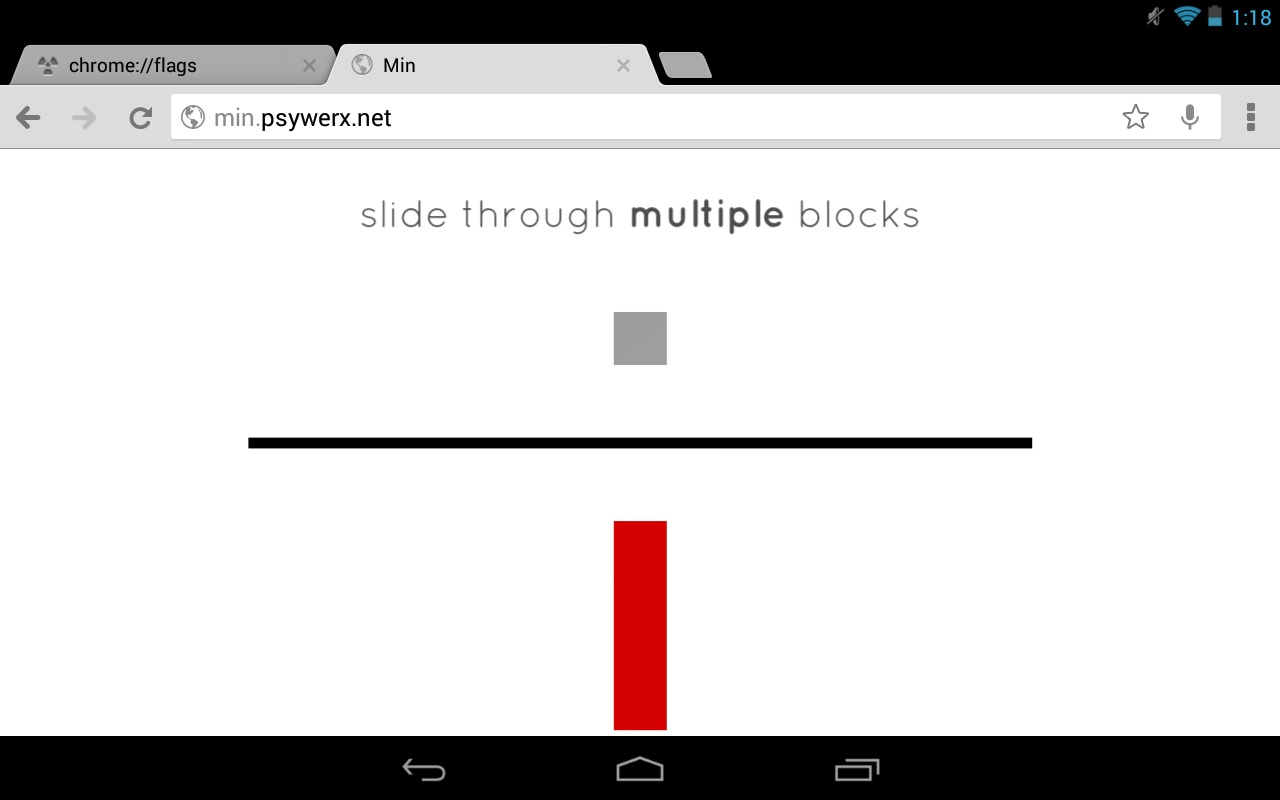
\includegraphics[width=12cm]{pic/min-chrome.png}
\end{center}
\caption{Delovanje igre v mobilnem brskalniku Chrome.}
\label{minchrome}
\end{figure}

\section{Primer OGRE (C++)}


%Primer Min je bil narejen s pomočjo knjižnice LibGDX. Za svoje delovanje izrablja %zmoglivosti OpenGL ES 2.0. 


